\documentclass[12pt, varwidth, border={20mm 5mm 5mm 20mm}]{standalone}
\usepackage{tikz}
\usepackage{amsmath}
\usepackage[a4paper, portrait, margin=1cm]{geometry}
\begin{document}
\section*{First Class Lever mechanical advantage}
\begin{minipage}{0.5\textwidth}
    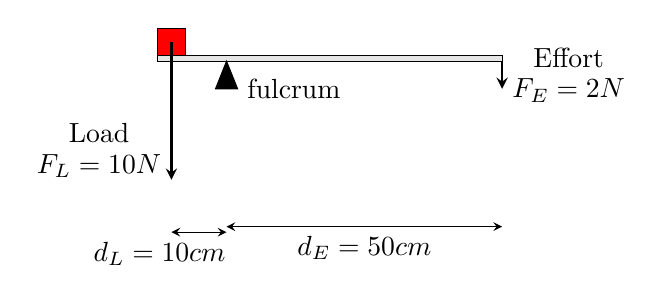
\begin{tikzpicture}[scale=0.7,>=stealth]
        % First class lever
        % rod
        \draw[fill=gray!20] (-0.25,0) rectangle (6,0.1);
        %fulcrum
        \draw[fill=black] (0.8,-0.5) -- (1.2,-0.5) node[right] {fulcrum} -- (1.0,0) -- cycle;
        %load
        \draw[fill=red] (-0.25,0.1) rectangle (0.25,0.6);
        \draw[->,thick] (0.0,0.35) -- (0.0,-2.15) node[midway,left,yshift=-0.5cm,align=center] {Load \\\\[-3ex] $F_L = 10N$};
        %effort
        \draw[->,thick] (6,0.0) -- (6,-0.5) node[midway,right,align=center] {Effort \\\\[-3ex] $F_E = 2N$};

        % Distance markers
        \draw[<->] (1,-3.0) -- (6,-3.0) node[midway,below,align=center] {$d_E= 50cm$};
        \draw[<->] (0,-3.1) -- (1.0,-3.1) node[midway,below,xshift=-0.5cm,align=left] {$d_L = 10cm$};
    \end{tikzpicture}
\end{minipage}%
\hfill
\begin{minipage}{0.3\textwidth}
    \begin{align*}
        % ma
         m.a.&=\frac{F_L}{F_E}=\frac{10N}{2N}=5 \\\\
         m.a.&=\frac{d_E}{d_L}=\frac{50cm}{10cm}=5
    \end{align*}
\end{minipage}
\end{document}